\section{Problem Formulation}
\label{sec:formulation}
\subsection{Single Base Transceiver Station (BTS)}
Power consumed by a BTS, as a function of traffic load, can be
well approximated as a linear curve with a non-zero
y-intercept~\cite{Peng:2011:BTSSaving:Mobicom} given as
$P_1+l(P_2-P_1)/t_{max}$. Here $P_1$ and $P_2$ are the power
consumption at no load and full load, respectively, $l$ is the
number of calls presently being handled, and $t_{max}$ is the
maximum number of calls that can be handled.

Let $\delta$ be the traffic threshold at which the \textit{BTS
power savings} is applied (i.e., when BTS deactivates some TRXs
moving into low-power mode). Since all TRXs are identical, the
per call increase in power consumption, and hence the slope of
the power consumption profile in Fig.~\ref{fig:powermodel},
remains the same whether or not some TRXs are deactivated. As
also indicated in Fig.~\ref{fig:powermodel}, the no-load power
consumption drops to $P_1-\gamma$ in the low-power mode, where
$\gamma$ is a constant that depends on the equipment type and
the number of TRXs deactivated.

If $x$ is an indicator variable which is 1 when \textit{BTS
power savings} is applied, and $0$ otherwise, then the BTS
power consumption may be given by $P_1+l(P_2-P_1)/t_{max} -
(1-x)\gamma$, also indicated in Fig.~\ref{fig:powermodel} by
the piecewise linear solid line.

\begin{figure}
\centering
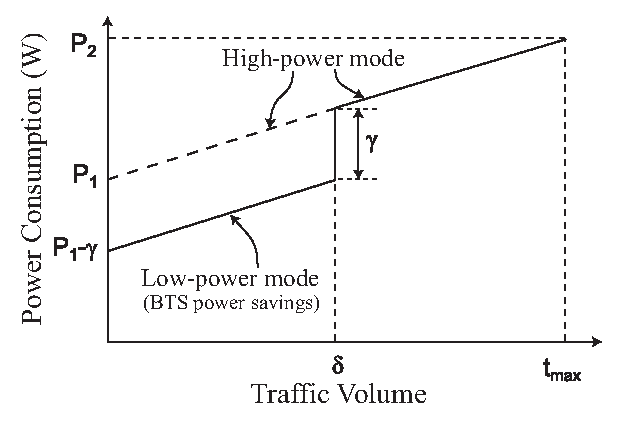
\includegraphics[width=0.28\textwidth]{figures/powermodel.eps}
\caption{BTS power consumption model. Low-power (BTS power savings) mode is optional and kicks in at low loads.}
\label{fig:powermodel}
\end{figure}

\subsection{Multi-BTS Cellular Setting}
Consider an area with $n$ active callers being served by $m$ BTSs.
We introduce indicator variable $w_{i,j}$, which is $1$ if call
$i$ \textit{is being} handled at BTS $j$ and $0$ otherwise. We
assume availability of an $n\times m$ matrix whose entry
$c_{i,j}$ is $1$ if caller $i$ \textit{can be} served through
BTS $j$ without exceeding the uplink or downlink budgets.
This information can be extracted by the data periodically
transmitted by each MS comprising the received signal strength
from nearby BTSs during a call. We also introduce indicator
variable $x_j$, which is $1$ if BTS $j$ is operating in
high-power mode (i.e., without \textit{BTS power savings}) and
$0$ otherwise. Using these variables and parameters, we can
formulate an optimization problem to minimize the total power
consumption over the network as:
\begin{align}
\textit{minimize} \quad \sum_{j=1}^{m} \left[
P_1+\sum_{i=1}^{n}\frac{w_{i,j}(P_2-P_1)}{t_{max}}-(1-x_j)\gamma
\right]
\end{align}
subject to the following constraints:
\begin{align}
& \sum_{j=1}^m w_{i,j} = 1 \qquad \forall i \\
& w_{i,j} \leq c_{i,j} \qquad \forall i, j \\
& \sum_{i=1}^nw_{i,j}-\delta \leq Mx_j \qquad \forall j%\\
\end{align}
\begin{align}
& \sum_{i=1}^n w_{i,j} \le t_{max} \qquad \forall i \\
%\end{align}
%\begin{align}
& w_{i,j}, x_j \in {0,1} \qquad \forall i, j%\\
%x_j \in {0,1}
\end{align}

The objective function is a simple generalization from the case
of one BTS. The first constraint ensures that no active call is
dropped just to save on power. The second constraint secures
the uplink budget by ensuring that no call is routed to a BTS
that can not handle it. The third constraint picks the correct
value for the decision variable $x_j$. The fourth constraint is the capacity constraint on all BTSs, while the last
constraint is the binary value constraint on the decision
variables.

The above optimization problem is a Binary Integer Program
(BIP), which is NP-Hard. It is intractable to solve it for an
operator's entire network, but solving it for a subset of the
network will provide some estimates of the amount of energy
savings possible using Low-Carb. Deployment to large operator
networks would require approximation algorithms.